\let\negmedspace\undefined
\let\negthickspace\undefined
\documentclass[journal]{IEEEtran}
\usepackage[a5paper, margin=10mm, onecolumn]{geometry}
%\usepackage{lmodern} % Ensure lmodern is loaded for pdflatex
\usepackage{tfrupee} % Include tfrupee package

\setlength{\headheight}{1cm} % Set the height of the header box
\setlength{\headsep}{0mm}     % Set the distance between the header box and the top of the text

\usepackage{gvv-book}
\usepackage{gvv}
\usepackage{cite}
\usepackage{amsmath,amssymb,amsfonts,amsthm}
\usepackage{algorithmic}
\usepackage{graphicx}
\usepackage{textcomp}
\usepackage{xcolor}
\usepackage{txfonts}
\usepackage{listings}
\usepackage{enumitem}
\usepackage{mathtools}
\usepackage{gensymb}
\usepackage{comment}
\usepackage[breaklinks=true]{hyperref}
\usepackage{tkz-euclide} 
\usepackage{listings}
% \usepackage{gvv}                                        
\def\inputGnumericTable{}                                 
\usepackage[latin1]{inputenc}                                
\usepackage{color}                                            
\usepackage{array}                                            
\usepackage{longtable}                                       
\usepackage{calc}                                             
\usepackage{multirow}                                         
\usepackage{hhline}                                           
\usepackage{ifthen}                                           
\usepackage{lscape}
\begin{document}

\bibliographystyle{IEEEtran}
\vspace{3cm}

\title{2.7.24}
\author{EE25BTECH11012-BEERAM MADHURI}
% \maketitle
% \newpage
% \bigskip
{\let\newpage\relax\maketitle}

\renewcommand{\thefigure}{\theenumi}
\renewcommand{\thetable}{\theenumi}
\setlength{\intextsep}{10pt} % Space between text and floats


\numberwithin{equation}{enumi}
\numberwithin{figure}{enumi}
\renewcommand{\thetable}{\theenumi}
\textbf{Question}:\\
If the vertices of a triangle are $(1,-3)$, $(4, p)$ and $(-9, 7)$ and its area is $15$ sq. units. Find the value(s) of $p$.\\
\textbf{Solution: }
let $\mathbf{A}$, $\mathbf{B}$ and $\mathbf{C}$ be the vectors such that:
\begin{table}[h!]
    \centering
    \begin{tabular}[12pt]{ |c| c|}
    \hline
    \textbf{Variable} & \textbf{value}\\ 
    \hline
    \textbf{$A$} & $\myvec{1\\-3}$\\
    \hline
 \textbf{$B$} & $\myvec{4\\p}$\\
    \hline
 \textbf{$C$} & $\myvec{-9\\7}$\\
    \hline
    \end{tabular}
    \caption{Variables used}
    \label{table 2.7.24}
\end{table}\\
given {ar}($\Vec{A}$$\Vec{B}$$\Vec{C}$) = $15$ sq.units
\begin{align}
\text {ar}(\Vec{A}\Vec{B}\Vec{C}) = \frac{1}{2} \| (\vec{B}-\vec{A}) \times (\vec{C}-\vec{A}) \| \\
= \frac{1}{2} \| \vec{B} \times (\vec{C}-\vec{A}) - \vec{A} \times (\vec{C}-\vec{A}) \|\\
= \frac{1}{2} \|\vec{B} \times \vec{C} - \vec{B} \times \vec{A} - \vec{A} \times \vec{C} + \vec{A} \times \vec{A} \|\\
= \frac{1}{2} \| \vec{B} \times (\vec{C}-\vec{A}) - \vec{A} \times \vec{C} \|\\
\end{align}
Substituting the values of $\Vec{A}$,  $\Vec{B}$,  $\Vec{C}$
\begin{align}
{ar} (\Vec{A}\Vec{B}\Vec{C})= 5|p+6| = 15\\
|p+6| = 3\\
P=-3 , -9
\end{align}
Hence, Value of $p$ is $-3$ , $-9$.

\begin{figure}[H]
    \centering
    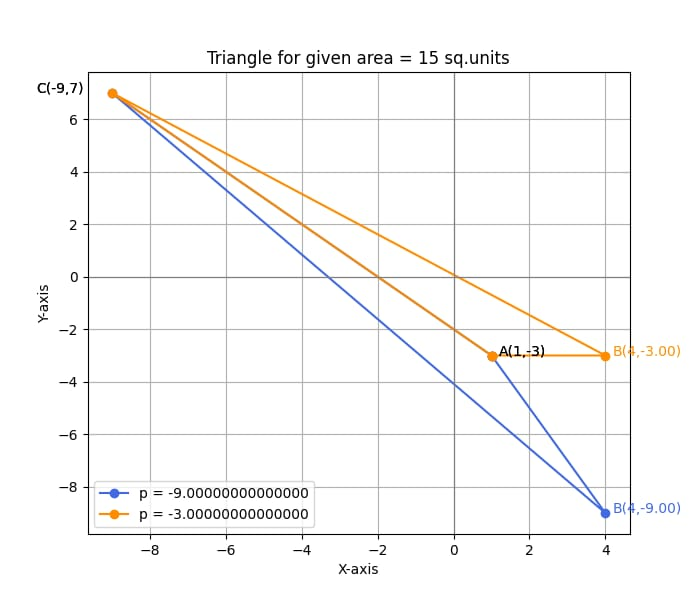
\includegraphics[width=0.75\columnwidth]{figs/graph-1.png}
    \caption{Triangle ABC}
    \label{fig:placeholder}
\end{figure}
\end{document}